\documentclass[a4paper]{article}
\usepackage[english]{babel}
\usepackage{fullpage}
\usepackage{graphicx}
\usepackage[utf8]{inputenc}
\usepackage{listings}
\usepackage{parskip}
\usepackage{xcolor}
\usepackage{fancyvrb}
\usepackage{csquotes}
\usepackage{biblatex}
\addbibresource{bib.bib}

\usepackage{tikz}
\usetikzlibrary{positioning}
\lstdefinelanguage{JavaScript}{
    morekeywords={abstract,arguments,boolean,break,byte,case,catch,char,const,continue,debugger,default,delete,do,double,else,eval,false,final,finally,float,for,function,goto,if,implements,in,instanceof,int,interface,let,long,native,new,null,package,private,protected,public,return,short,static,switch,synchronized,this,throw,throws,transient,true,try,typeof,var,void,volatile,while,with,yield},
    showstringspaces=false,
    morestring=[b]{'},
    morestring=[b]{"},
    basicstyle={\ttfamily},
    commentstyle=\color[rgb]{0.9,0.1,0.1},
    keywordstyle=\color[rgb]{0,0.5,0},
    keywordstyle=[2]\color{blue},
    stringstyle=\color{orange},
    numbers=left,
    numberstyle=\small,
    columns=fixed
}
\lstdefinelanguage{TypeScript}[]{JavaScript}{morekeywords={break,case,catch,class,const,continue,debugger,default,delete,do,else,enum,export,extends,false,finally,for,function,If,import,in,istanceOf,new,null,return,super,switch,this,throw,true,try,typeOf,var,void,while,with,as,implements,interface,let,package,private,protected,public,static,yield,any,boolean,constructor,declare,get,module,require,number,set,string,symbol,type,from,of}}
\PassOptionsToPackage{hyphens}{url}

\usepackage{hyperref}

\useshorthands{"}
\defineshorthand{"-}{\babelhyphen{nobreak}} % en hyphen som inte linebreakar

\title{\Huge Vikings of Vader \\ \Large The Best Multiplayer Game of the Century \\[1em] \large Software Engineering Project 1DL650}

\author{Staffan Annerwall \and August Dixelius \and Pontus Eriksson \and Daniel Jansson \and Carl Nordström \and Erik Rimskog}
\date{\today}

\begin{document}

\maketitle

\begin{abstract}
With the Covid"-19 pandemic, people are more alone than before. Not being able to see their close ones due to restrictions can be tough. This report describes the creation of a survival multiplayer shooter game. It dives down into lag compensation and how we managed to work together even though we could not meet in person.
To create this game we used some third-party libraries like a physics engine to move our characters and a graphics library for drawing everything. We connected all clients together via a server. To make the enemies move we have implemented an AI, and to make the game feel robust and responsive while playing we implemented client-side prediction.


\end{abstract}

\newpage

\tableofcontents
\newpage

\section{Introduction}
% Introduction (Scope statement)
% Problem formulation

With the Covid"-19 pandemic, people are more alone than before~\cite{web:loneliness}. Not being able to see their close ones due to restrictions can be tough. Finding activities to do when you can not meet others in person can be a hard task. This project seeks to create one such activity, specifically a web browser game.
Creating a game for web browsers is convenient for the users because they do not have to install anything on their own computers. The easy access of the game is also one of the most important things with our game since we want everyone, even those with limited computer knowledge to easily be able to access and play the game. The only thing needed to start the game is to enter an URL in a browser and the game is up and running.

% The game we created is a multiplayer game where one or more players travel to a previously peaceful planet where only peace and joy had been seen for centuries. Unfortunately, the planet has been overthrown by the evil organization ``Vikings of Vader'' (VoV), a gang of seemingly endless amount of criminals, all of which has done unspeakable things. It is up to the players to fend off these delinquents using their various weapons of destruction and restore order in the galaxy. May the Force be with them!

We created a multiplayer shooter game where the players take the roles of Vikings of Vader (VoV), an elite group of warriors that serve the evil Vader. The vikings are carrying out Vader's commands on a desolate planet when they are overrun by a seemingly endless amount of rebel scums. The vikings are away from their ship and cannot escape, so they must survive for as long as possible and take as many rebel scums to the grave with them as possible.

To create this game we used some third-party libraries like a physics engine to move our characters around and a graphics library for drawing everything. We connected all clients together via a server and made sure that the connection was reliable (Sections \ref{sec:softwaredesign} and \ref{sec:sendinginputs}). To make the enemies move we have implemented an AI that follows the closest player (see Section~\ref{sec:eai}). We have also animated our player characters, and the game map was created from scratch (Section~\ref{sec:gam}). To make the game feel robust and responsive while playing we implemented client-side prediction (Section~\ref{sec:csp}). Also, we created a compressed format for sending data between client and server (Section~\ref{sec:compressing}). Finally we created a simple lobby for connecting players together (Section~\ref{sec:lobby}).

\section{Gameplay Description}\label{sec:gameplay}
Each player connects to a lobby (a waiting room) and waits until all connected players are ready to start.
When everyone is ready the game starts and the view changes to display the game arena and everyone can see their own playable characters, like in Figure~\ref{fig:game}.

The players can use the arrow keys to move in one of eight different directions---north, north-east, east, south-east, etc.---or stand still if no key is pressed. The players have a ranged weapon which they can fire in the direction they are facing by pressing the space bar. If the fired projectile hits an enemy, that enemy takes damage. You can not damage your fellow players or damage the walls by firing at them.

An enemy will damage the players by colliding with them, and they will chase the nearest players around the map. The maps are quite big so you can stay at a distance far from the enemies in the beginning, but when there is a high number of enemies you will have to play smartly. As seen in Figure~\ref{fig:game2}, the player is about to be overrun by the enemy force and has to be creative to be able to survive.

Enemies will spawn in groups, so-called ``waves'', and a new wave will spawn when all the enemies of the most recent wave have been vanquished. Each wave will be more difficult than the previous, by spawning more and stronger enemies. There is no final wave; the players has to survive for as long as possible. When a player loses all of its health, the player dies. The game ends when all players are dead. When a wave is completed, i.e.\@ when all enemies have been killed and no more enemies are spawning, all dead players are revived and all living players return to full health before the next wave begins.

\begin{figure}[!ht]
    \centering
    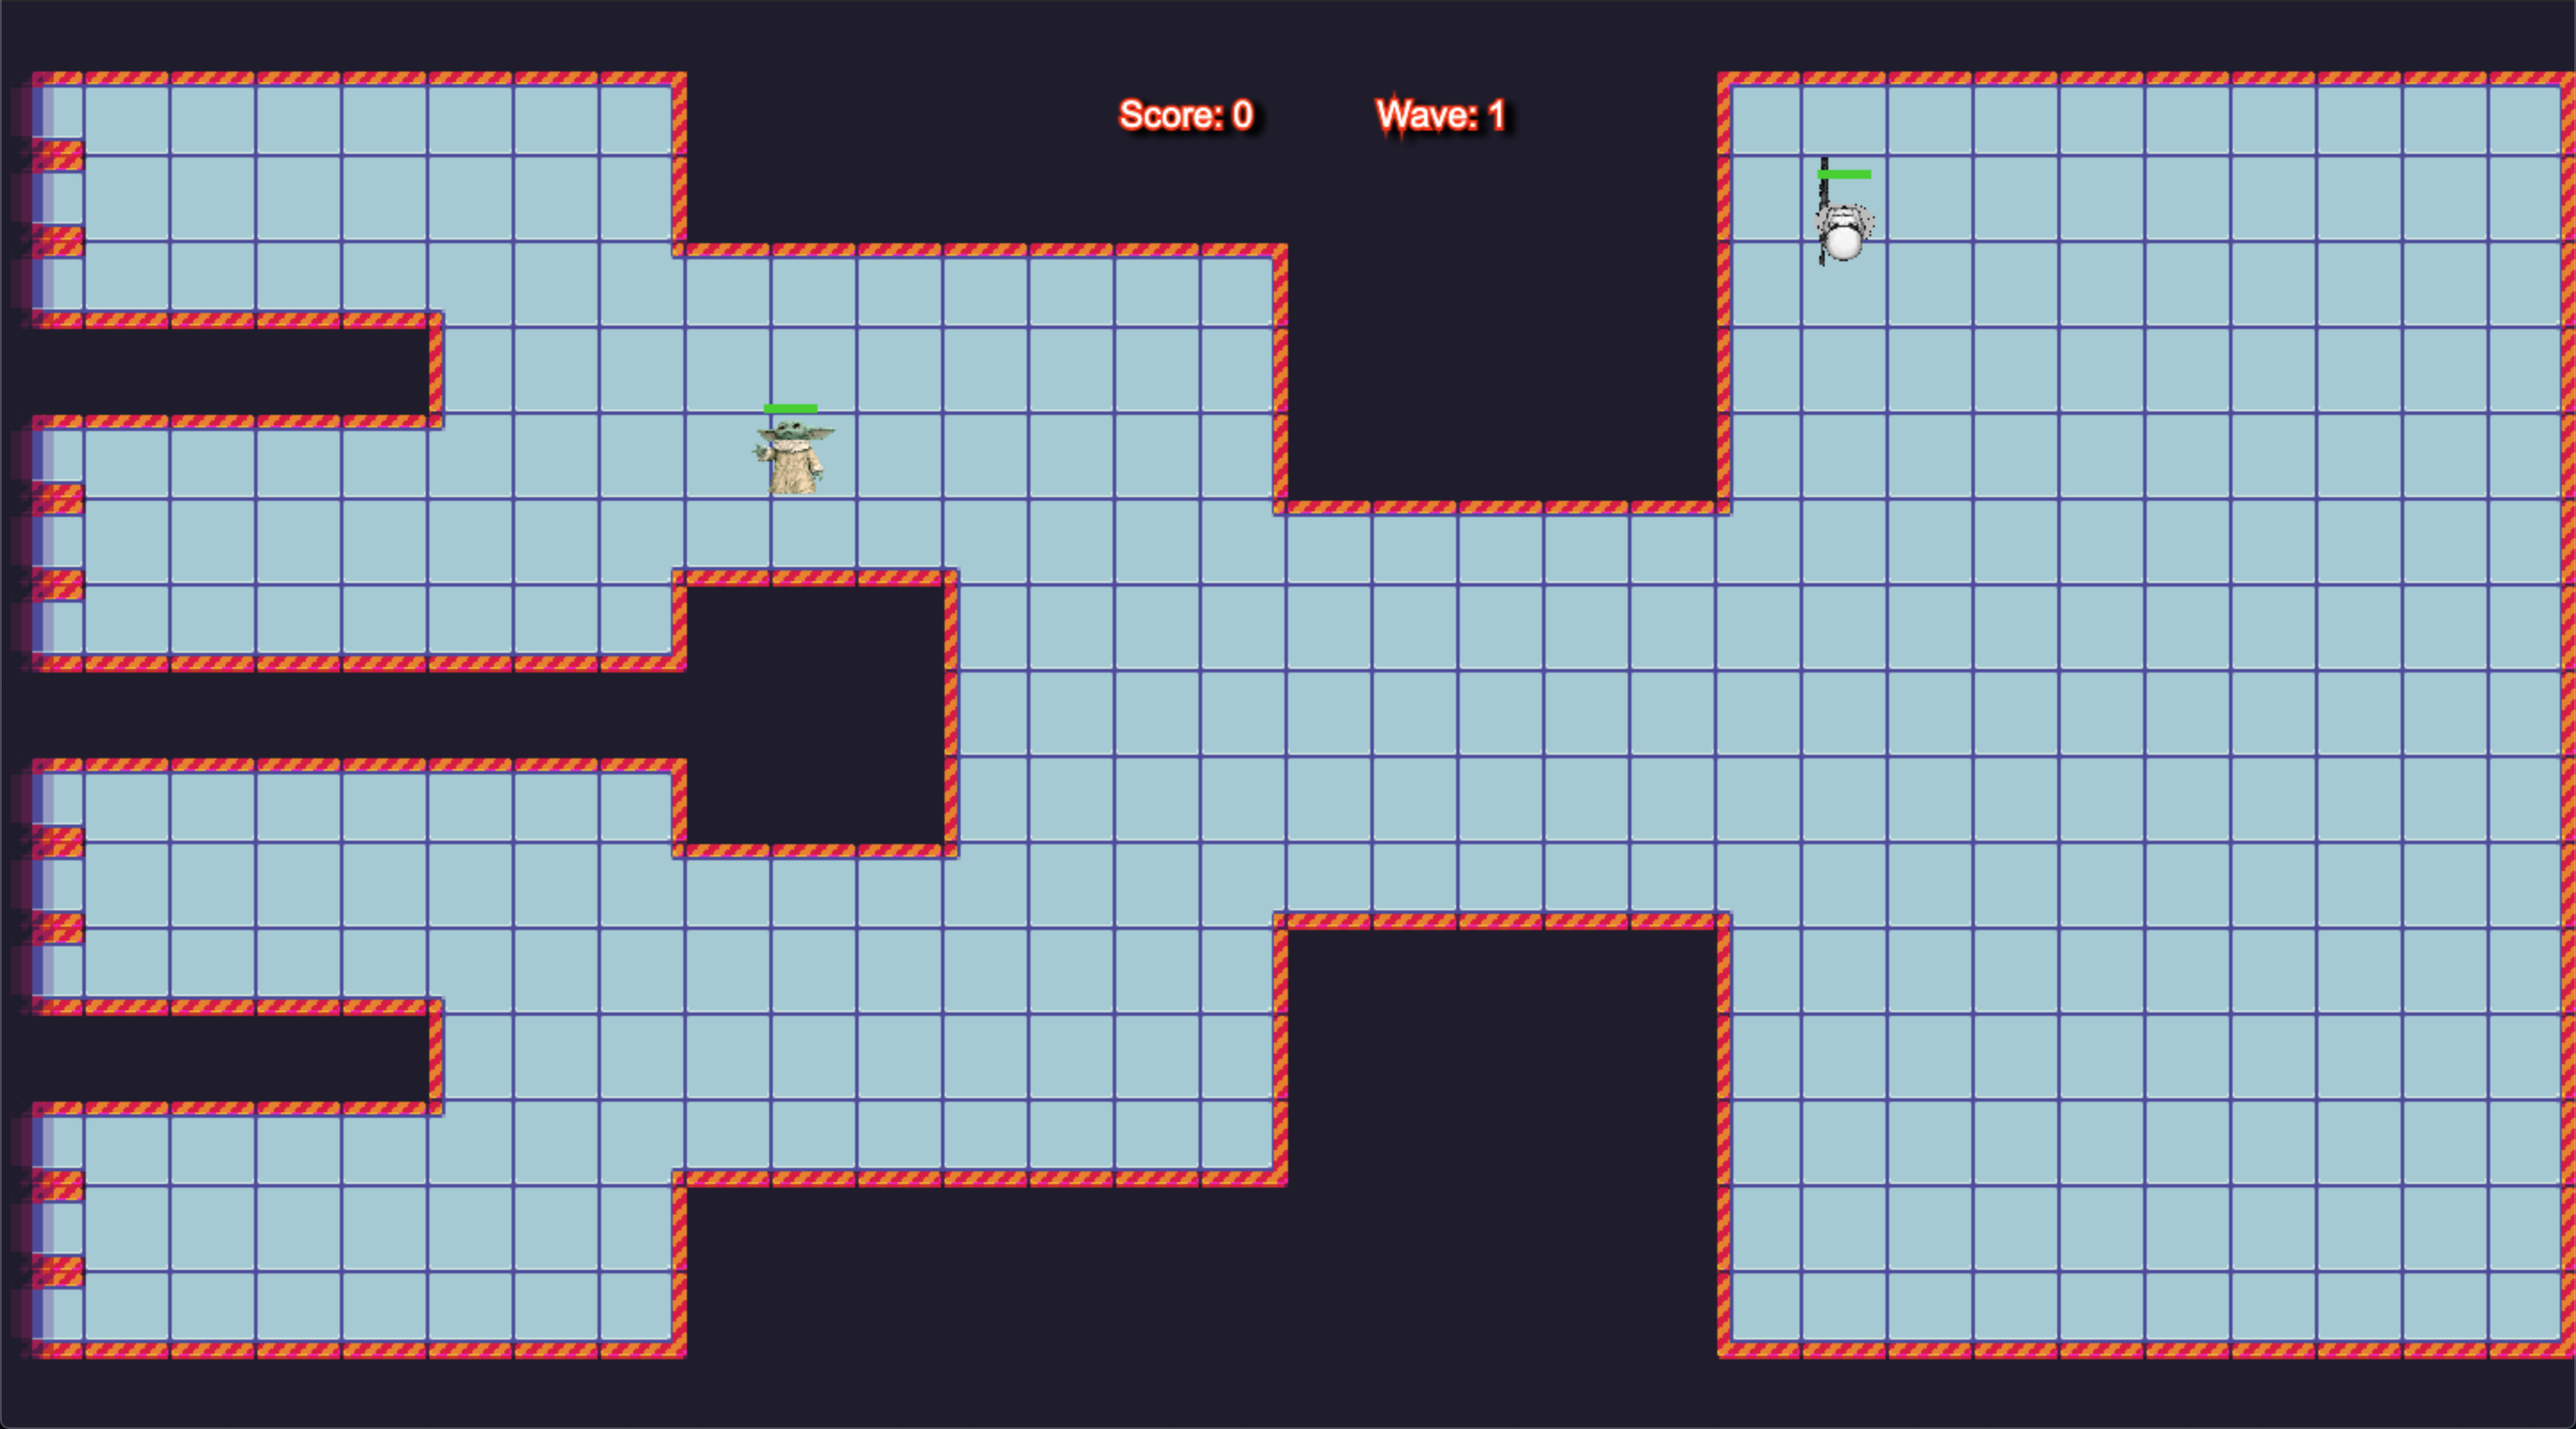
\includegraphics[width=0.9\textwidth]{pics/beginning.png}
    \caption{A screenshot of the game in action. The white character is the player and the green ones are the enemies.}
    \label{fig:game}
\end{figure}

\begin{figure}[!ht]
    \centering
    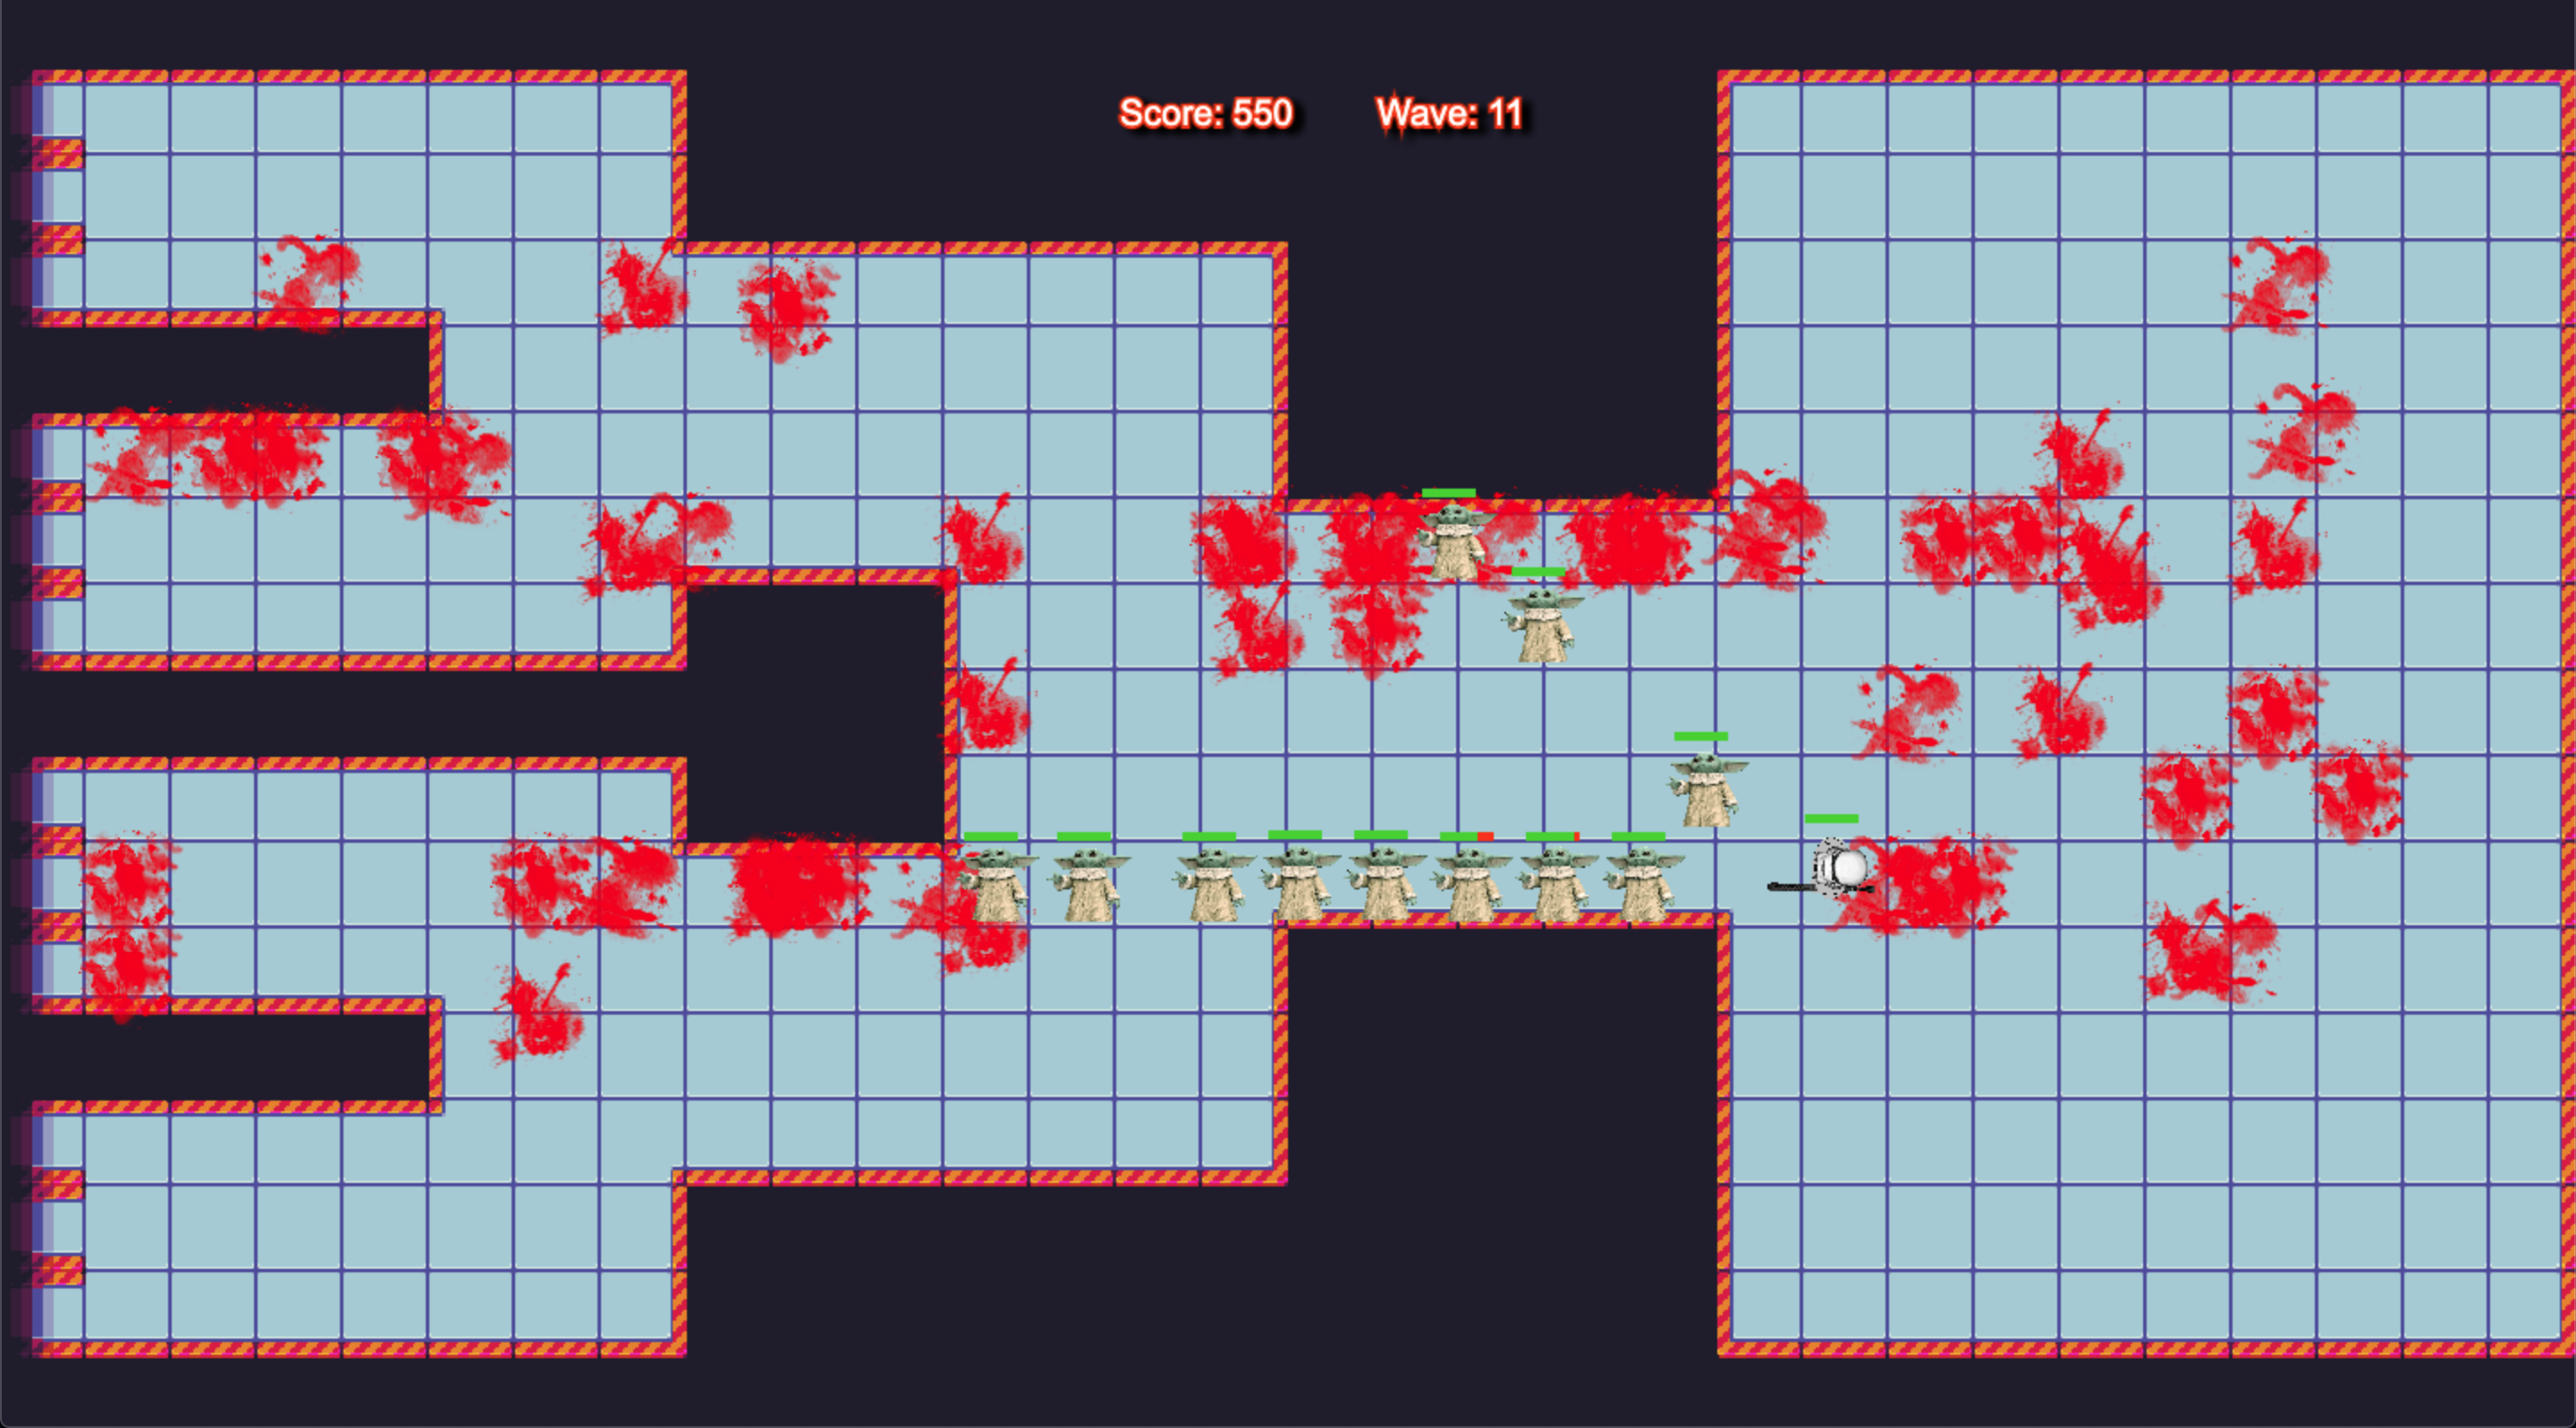
\includegraphics[width=0.9\textwidth]{pics/pushedBack.png}
    \caption{A screenshot of the game in action.}
    \label{fig:game2}
\end{figure}

%\section{Usage}\label{sec:usage}
% User documentation of the software, including installation instructions, as appropriate.
%The game requires two parts to run, one server and one or more clients. The clients run the game in a web browser while the server runs in Node.js. With Node installed, the server can be started with the command \texttt{npm run dev}. Clients must connect to the server; the default port is 3000.

\section{Requirements}
% Requirements on the software

For the game to be as easy to play as possible, we chose to make a game played in web browsers. This means that the players do not need to install anything, and the amount of setup required before playing is low (except for running a server, which requires a little bit of work).

We wanted to support at least 4 players playing together in order to allow people to have fun together, if they so please. The game theoretically supports an unlimited number of players, but we have only tested it with at most 6 players. We believe that network packet size and the CPU performance are bottlenecks as the number of players grows.

To increase variability, we wanted multiple maps that the players could choose to play on. We initially set out to have at least 2 playable maps. In the end, we had exactly 2 working maps.

To avoid starting the game too early, for example before all players have joined, we used lobbies. A lobby in our game is the start screen you connect to where the players wait for other players to get ready before the actual game starts. After connecting, the players are given a button to tell the server whether they are ready to play or not. The game starts when all connected players have pressed the button.

We wanted the enemies to spawn periodically in waves. This was to give players brief breaks while playing and to give a clear indication of progress.

The enemies get stronger over time in order to make the game more difficult as the players progress. We had ideas for the players to get stronger as well, for example with better weapons, but this is not implemented in the final game.

Latency and packet loss are largely inevitable for communication over the Internet, so we wanted to make the game work well with high latency and some packet loss.

\section{Related Work}
There have been many types of similar games that we have taken inspiration from, such as boxhead, slither.io, agar.io and Counter-Strike.

\textbf{Boxhead} is a browser game that belongs in the same genre, a shooter game where you defend yourself against waves of enemies. It was created in 2006 by Sean Cooper and became fairly popular~\cite{boxhead}. In boxhead, as well as in our game you can move in eight directions, up, down, left, right and then combinations of these. A difference between VoV and Boxhead is that Boxhead only supports multiplayer on the same computer, while VoV supports multiplayer over internet. This is otherwise the sole inspiration for our game.

\textbf{Slither.io} and \textbf{agar.io} are more browser games that also are developed in JavaScript and have open lobbies that you can connect to via the browser~\cite{article:agar}. The games themselves are completely different from ours, but they have in common that they are multiplayer over the internet though. These games use websockets (TCP) for their communication~\cite{article:slither} while we use UDP, we discuss this under Section~\ref{sec:techs}. An easy-to-use UDP solution for browsers didn't really exist when these games were created~\cite{web:agario:webrtc}, but they work pretty well anyway. We wanted to try to use a newer solution, namely geckos.io~\cite{geckos}, and see how easy it is to create games in browsers nowadays with UDP support.

\textbf{Counter-Strike} is a completely different game from ours. It is a game created with the Source game engine, so this game is not run in the browser. We were heavily inspired by Counter-Strike's networking model, and they are doing a lot more things than us to compensate for network delays. What they are doing and how it works is described in a developer wiki page from Valve~\cite{web:valve:mp} and is summarized here:

\begin{description}
\item [Server and client] All players connect to each other and one is assigned the host (possible to have a dedicated server as well). The host is authoritative about what happens in the game. All clients are sending their keyboard inputs to the host and the host responds with state changes.
\item [Client-side (input) prediction] The client predicts how the host will update the game state. This reduces inputs lag, i.e.\@ how long it takes for something to happen after a key has been pressed.
\item [Game state snapshot] They are only sending what has changed in the game in their packets from the host.
\item [Lag compensation] All clients have slightly different position information for all players because of network delay. This can be problematic for important event like carefully aiming and shooting at someone. One client might think that a shot landed while another thinks he/she ran around a corner just before the shot. The host can revert itself temporarily to make it look exactly like it does on one of the clients to make better decisions.
\item [Interpolation] The host can send fewer state updates if the clients interpolate between states to make the experience smooth anyway. For example, the host might send states 20 times per second and the client can interpolate these to get 60 state updates per second.
\end{description}

Our game has a dedicated server, using one client as a host is not possible. We are also sending keyboard inputs from the client to the server and receiving states. We are sending whole states from the server, though, and not just the changes. Finally, the only delay mitigating method we are using is client-side prediction.

There are many more ways to sync a game state between nodes in a network. The main difference is what information each client is sending to the server. It is possible for each client to send its new position to the server and the server is broadcasting that to everyone else. The difficult thing is how to solve the conflicts in a good way when two clients are doing contradictory things. Sending keyboard inputs seemed to be the easiest since the game is only run in one place, and there is no need to synchronize multiple games.

% An overview of similar software or software that have inspired you.

\section{Method}
% Technical documentation of the software: Several sections describing the design, the tools you have been using and their purpose, database diagrams, models, components, integration.
% Testing/quality control methods
This section describes the process and technologies we used to develop our game, as well as more detailed descriptions of the resulting software architecture and implementation.

\subsection{Project Organization}
% Your project management approach including description of any tools used.
Organizing a project while not being able to meet in person due to the Covid"-19 pandemic has posed a lot of challenges, for example not being able to meet and work in person. At the start of the project we sat down and planned how we would structure it. We decided upon using Discord as our main source of communication. Discord is a tool that allows the users to create a server with many different text and voice channels. The voice channels have been used to simulate different rooms where different people can sit and work with each other, while also allowing others to simply pop by when they have a question. See Figure~\ref{fig:voice_channels}.

We adopted the kanban development method in organizing our work. As it was a shorter project, approximately ten weeks, a light weight organizational tool was fitting, as it added little overhead and still helped us organize our work. We had a scrum board on GitHub where we mainly used four different categories: ``Backlog'', ``To do'', ``In progress'' and ``Done'', see Figure~\ref{fig:project_board}. Here, every member could grab something from the ``To do'' column if they wanted something to do.

To organize the daily work we had a daily stand up meeting each day at 10:15 in one of the voice channels in Discord. Here everyone explained what they were going to do that day, and if someone was without a task the rest of the group helped that person to find something to do. Also if someone had encountered a problem, the rest of the group could help that person.

For keeping track of decisions that have been made like project diaries and other documents concerning the project, a Google Drive folder was set up. This enabled everyone to be able to share documents, keep them updated and edit them in real-time.

\begin{figure}
    \centering
    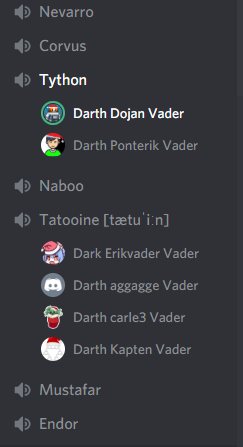
\includegraphics[width=0.4\textwidth]{pics/voice_channels.PNG}
    \caption{The team working in different voice channels in Discord.}
    \label{fig:voice_channels}
\end{figure}

\begin{figure}
    \centering
    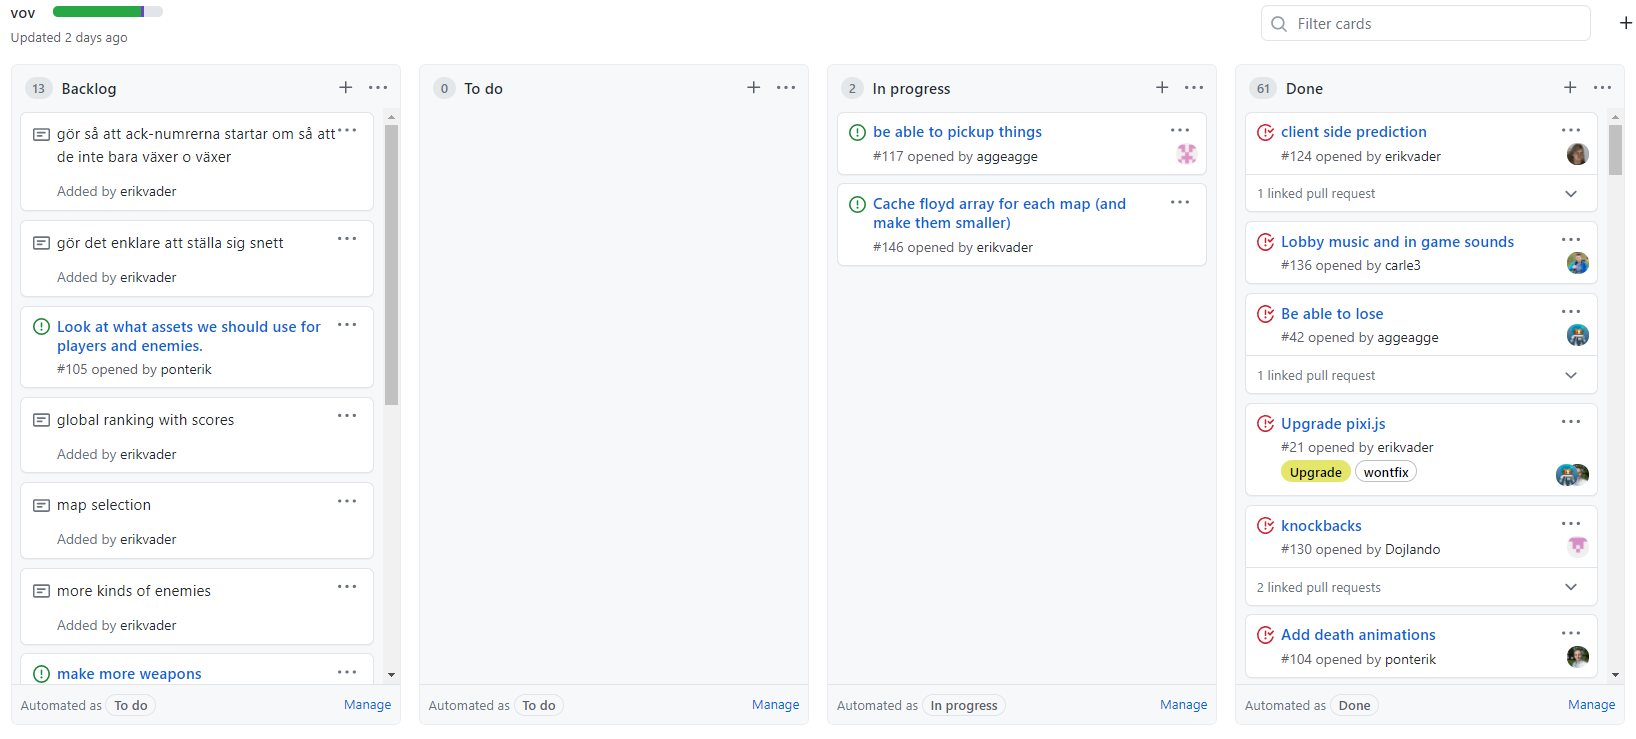
\includegraphics[width=1\textwidth]{pics/project_board.PNG}
    \caption{The project board where we organized our tasks.}
    \label{fig:project_board}
\end{figure}

\subsection{Tools}
% Here we give a brief description of the major tools that we have used.

We used GitHub~\cite{github} for hosting our source code and our kanban project board. It makes doing code reviews and coordination easier with features such as issues, brief descriptions of planned extensions or bugs in the software, and pull requests, a request for ``pulling'' additional code into the project.

Google Drive~\cite{drive} is a file sharing web service hosted by Google. We used this service to share all project files not related to the code, for example the project diaries, presentations, and progress reports.

\subsection{Technologies}\label{sec:techs}

This section covers the technologies we used to create the game.

TypeScript~\cite{typescript} is an extension of JavaScript that offers a strong type system among other things on top off JavaScript. We think writing code becomes significantly easier when you can reason about types, and can have a compiler making sure that typing rules are followed.

As an example, consider a function that takes an array of strings as an input and returns all strings concatenated into a single string. In JavaScript, this function would have the signature shown in Listing~\ref{lst:javascript}. Looking at the signature, it is not clear what \texttt{items} is or what the return type of the function is. In TypeScript, the function signature would be the one shown in Listing~\ref{lst:typescript}. Here, it is shown that \texttt{items} is an array of strings, and that the function returns a string, using syntax similar to other programming languages like Java. Another benefit with TypeScript is that the compiler can check that the typing rules are followed, e.g.\@ that the function \texttt{concatenate} in the previous example returns a string, which is expected.

\begin{lstlisting}[language=JavaScript,label=lst:javascript,numbers=none,caption={An example of a JavaScript function signature. The corresponding TypeScript signature is shown in Listing~\ref{lst:typescript}.}]
function concatenate(items)
\end{lstlisting}

\begin{lstlisting}[language=TypeScript,label=lst:typescript,numbers=none,caption={An example of a TypeScript function signature. The corresponding JavaScript signature is shown in Listing~\ref{lst:javascript}.}]
function concatenate(items: string[]): string
\end{lstlisting}

The server runs in Node.js~\cite{nodejs}, which is a runtime for running JavaScript outside a browser. Because the clients were going to be written in JavaScript in order to run in web browsers, and because we wanted to re-use code between the clients and the server, we chose to use JavaScript for the server as well.

Geckos.io~\cite{geckos} is used for communication over UDP~\cite{rfc768} in web browsers. If TCP is used, any packet loss in the network may cause noticeable lag for the end-users as it will re-send packets if they do not arrive, which is less than ideal for real-time multiplayer games. With communication happening over UDP, a dropped packet will not delay future packets, leading to higher responsiveness and a better playing experience. It is not essential to receive every single state since each one often contain only very small changes, so losing some packets is not devastating. It is more important to receive the latest state as fast as possible.

For physics, we utilized the Planck.js 2D physics engine~\cite{planckjs}. Every player and enemy are represented as individual rigid bodies in a physics simulation, and the velocities of these bodies are modified depending on user input and collisions with the world or other characters. Shots fired from players are implemented as queries of the physics simulation. On each game update, the server runs the simulation for a brief period of time before broadcasting the new state to all clients. We also implemented client-side prediction, see Section~\ref{sec:csp}.

Graphics is a large part of games and we used PixiJS~\cite{pixijs} for creating textures from images and rendering animated sprites in a web browser. We also used PixiJS to play an audio file when certain events occur, for example when players take damage or an enemy is dying. We could have managed all graphics ourselves by manipulating an HTML canvas element, but using PixiJS has some advantages. For instance, it can render using WebGL which improves performance if the browser supports it. It also allows us to use a more user-friendly high-level API with classes for sprites, among other things.

Tiled~\cite{tiled} is an open-source editor for creating tile-based game levels/maps. From a tilesheet, an image with multiple tiles drawn after each other, you create a set of tiles. Using these tiles, you can place these tiles in a grid and in this way create a game world. Figure~\ref{fig:tiled} shows an example of the Tiled editor running with a game map open for editing.

Piskel~\cite{piskelapp} is an online tool for creating animated sprites. An animated sprite is a collection of frames that can be played after one another to create the illusion of a picture moving. Using these, it is possible to play a walking animation when the player is moving.

% We used Overleaf for this final report. It is an online collaborative \LaTeX{} editor, similar to Google Docs.

\begin{figure}[!hb]
    \centering
    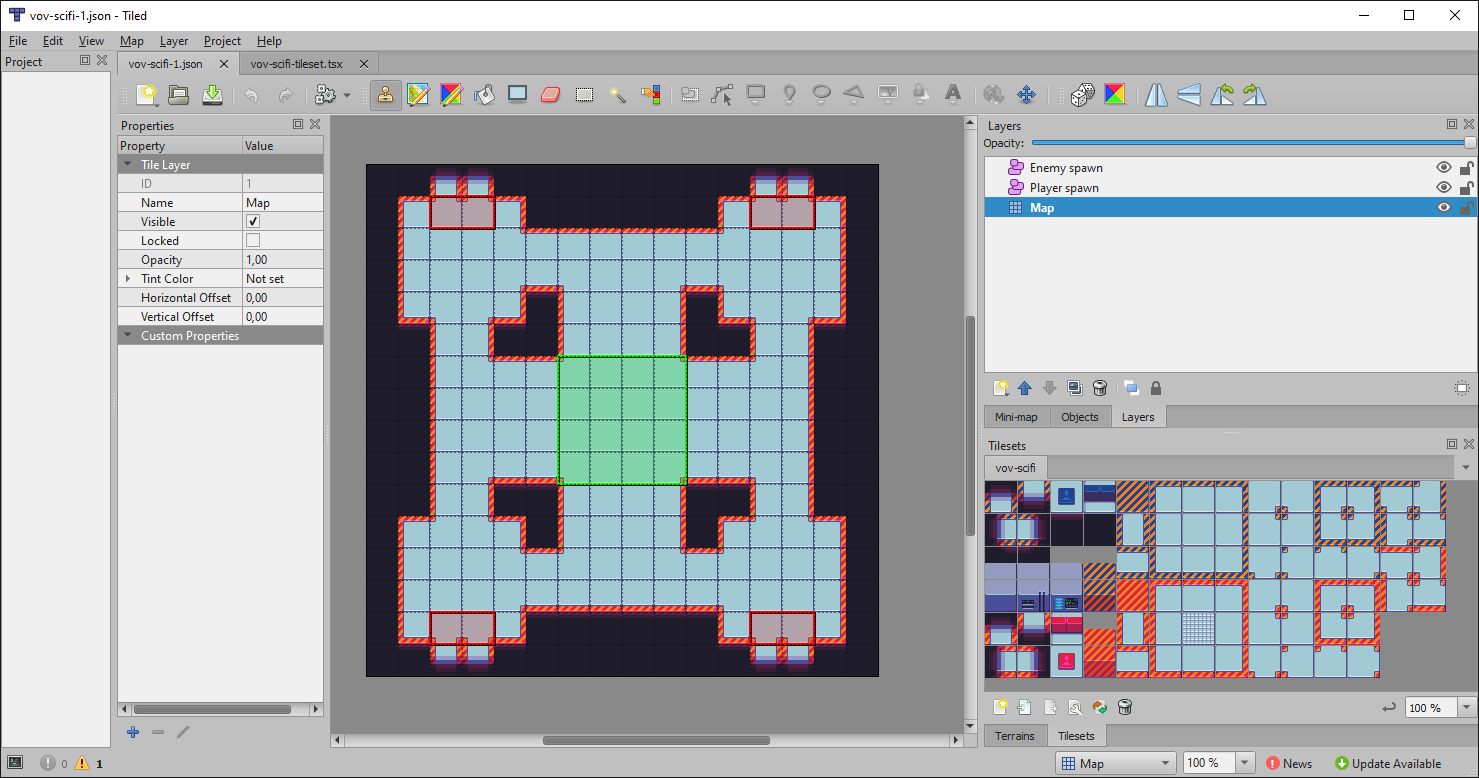
\includegraphics[width=\linewidth]{pics/tiled.png}
    \caption{The Tiled editor running with a game map open for editing. The tileset is visible in the bottom-right corner.}
    \label{fig:tiled}
\end{figure}

\subsection{Software Design}\label{sec:softwaredesign}
The software is using a server-client model (illustrated in Figure~\ref{fig:client-server}). The server does all the computations and keeps track of the game states while the clients render what the server has decided. A game state is the state of a game at a given time, for example it contains the positions and directions of all players and enemies. This avoids the problem of out-of-sync game states between all clients as the server is the one with the final say. Every client sends keyboard inputs to the server, and the server will move the player according to that input and broadcast the updated game state to all the clients. This adds a noticeable delay as the character will not move until the server sends the updated state. To increase responsiveness of the application we are using movement prediction on the client (client-side prediction), which is explained in detail in Section~\ref{sec:csp}.

\begin{figure}[!ht]
    \centering
    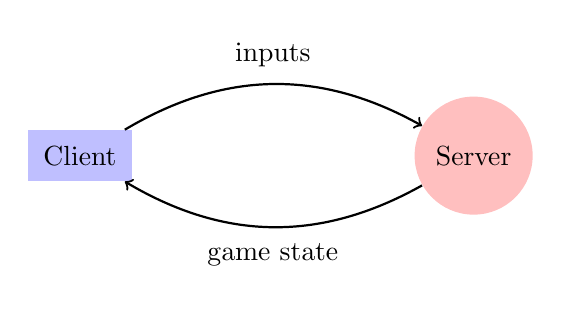
\begin{tikzpicture}[inner sep=2mm]
        \tikzset{client/.style={rectangle,fill=blue!25}};
        \tikzset{server/.style={circle,fill=red!25}};

        \node [client] (client) at (0,0) {Client};
        \node [server] (server) at (5,0) {Server};

        \draw [->,thick] (client) to [bend left] node [above,midway] {inputs} (server);
        \draw [->,thick] (server) to [bend left] node [below,midway] {game state} (client);
    \end{tikzpicture}
    \caption{A depiction of communications in a client–server model. The server manages the entire game logic and communicates with all clients individually. The clients receive and accept  whatever the server says and displays it, and send input information to the server.}
    \label{fig:client-server}
\end{figure}

To be able to do client-side prediction we had to be able to run all game logic (character movement, collisions, etc.) on both the server and the clients in a predictable and deterministic way. It must also be possible to revert the game to an earlier state and resume from there. We therefore modeled a game state as a list of all characters currently in the game (players and enemies), where each character keeps track of what position it has, which direction it is facing, how much health is has left, and so on. A state is combined with a set of keyboard inputs (one for each player) to get the next state, and the state is given to the display code which renders all characters.

There were no existing game libraries for the browser that provided the flexibility we needed. Most of them only ran on the client as a single player game and none had a game state that could be modified as we required. A game library typically consists of a display part that draws all graphics and a logic part that moves all characters and checks for collisions etc. We decided to use two separate libraries for these things, namely PixiJS and Planck.js, and integrate them ourselves with the requirements we had. Read more about those libraries in Section~\ref{sec:techs}.

As implementation we used an object-oriented approach where players, enemies, weapons, game maps, and even the game servers are structured as classes. We chose this partly because shared behavior is easily ``stuffed'' into abstract base classes that concrete sub-classes can inherit, and partly because it is a convenient paradigm that we were all familiar with from the start. In order to keep the code base from becoming a tangled mess, we attempted to achieve a code base with low coupling between classes and high cohesion inside classes.

\subsubsection{Client-Side Prediction}\label{sec:csp}
\begin{figure}[!ht]
    \centering
    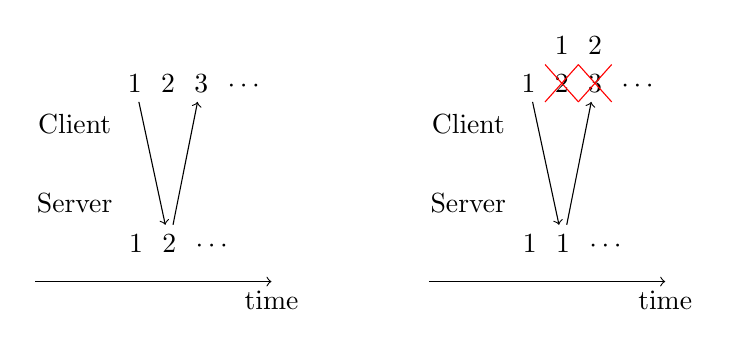
\begin{tikzpicture}
        % hidari 左
        \node (client1) at (0,0) {Client};
        \node (c11) [above right=1pt and -1pt of client1] {1};
        \node [above right=1pt and 11pt of client1] {2};
        \node (c13) [above right=1pt and 23pt of client1] {3};
        \node [above right=1pt and 35pt of client1] {$\cdots$};

        \node (server1) at (0,-1) {Server};
        \node [below right=1pt and -1pt of server1] {1};
        \node (s12) [below right=1pt and 11pt of server1] {2};
        \node [below right=3pt and 23pt of server1] {$\cdots$};

        \draw [->] (c11) -- (s12);
        \draw [->] (s12) -- (c13);
        \draw [->] (-0.5, -2) -- (2.5, -2) node [below] {time};

        % migi 右
        \node (client2) at (5,0) {Client};
        \node (c21) [above right=1pt and -1pt of client2] {1};
        \node (c22) [above right=1pt and 11pt of client2] {2};
        \node (c23) [above right=1pt and 23pt of client2] {3};
        \node [above right=1pt and 35pt of client2] {$\cdots$};

        \node [above=0pt of c22] {1};
        \node [above=0pt of c23] {2};

        \node (server2) at (5,-1) {Server};
        \node [below right=1pt and -1pt of server2] {1};
        \node (s22) [below right=1pt and 11pt of server2] {1};
        \node [below right=3pt and 23pt of server2] {$\cdots$};

        \draw [->] (c21) -- (s22);
        \draw [->] (s22) -- (c23);
        \draw [red] (c23.north west) -- (c23.south east) (c23.north east) -- (c23.south west);
        \draw [red] (c22.north west) -- (c22.south east) (c22.north east) -- (c22.south west);
        \draw [->] (4.5, -2) -- (7.5, -2) node [below] {time};
    \end{tikzpicture}
    \caption[asd]{Examples of the two main situations that can happen when the server responds. The numbers represent some kind of position, for example an x-coordinate. The client's view of this coordinate is shown on the top and the server's view is shown on the bottom. This position is increased by 1 each update and each update is represented by going to the right on the time axis (horizontal). For example, the client in the left example has the position of 1 initially, on the next update it has position 2 and on the last update it has a position of 3. The arrows represent messages sent over the network, the delay in these examples are exactly 1 update long.

    In the left example, the client sends an input to increase the x-coordinate to the server. It predicts that it will be able to do so and increases its own position by one. The server receives this input and decides that this coordinate can indeed be increased by one, and sends the updated state back to the client. The client then checks which input caused this state (the inputs are numbered) and backtracks in its state history and compares both positions. In this case, the value in both of them is 2, so the client knows that it predicted correctly and it does not need to correct for anything. The client can discard its history up to that point since the previous states are no longer needed.

    In the right example, the same thing happens except that the server \emph{does not} increase the position for some reason. When the client receives this position back it sees that it predicted incorrectly since $1 \ne 2$. The client must now correct itself and re-predict up to the point it was at before.}
    \label{fig:csp}
\end{figure}

To remove the potentially big delay when moving a character we used something called client-side prediction (CSP). The delay comes from the fact that it is the server that moves all characters. The client first sends its input to the server and the server responds with where the character moved to. This means that there are two network packets we have to wait for before we see the character move on the screen after we have pressed a key on the keyboard, and that delay can be very big depending on network conditions.

Client-side prediction removes this delay by predicting what the server will say. When the client sends an input it will also immediately move the character, making it appear as there is not any network delay. The client will also store the input for a potential re-predict when it predicted incorrectly, and it will also number it. When the server eventually responds the client finds the state associated to that input number and checks whether it predicted correctly or not. If the client predicted correctly, it then continues without interruption. If the client predicted incorrectly, it would then revert its state back to the first faulty state, replace it with the server's authoritative state and finally re-predict back until the state it was at. An illustration of these cases is shown in Figure~\ref{fig:csp}.

The network communications using UDP does not have any guarantees: packets may never arrive, arrive late or arrive in another order~\cite{rfc768}. Arriving late or never arriving is no big deal, the client will just predict a little bit further without any confirmation, which most likely does not have any big effect unless the delay is several seconds long. Arriving out of order is also fine since the older packets can be ignored, we only care about the latest state at all times.

We are not predicting everything about the game. Each client predicts its own character and all enemies, but not the other players. The client's own character is easy to predict since we always know all of its inputs, and the enemies are also easy to predict because they have a predictable movement pattern. The other players are difficult to predict since we do not know their inputs, at least not in real time since they are on different computers. So all the other players except yourself are in the past.

\subsubsection{Sending Inputs}\label{sec:sendinginputs}
To make sure that all inputs are received by the server is not straight forward when the network protocol is unreliable. The straight forward option of sending one input per packet is not possible since an input is forever lost if its corresponding packet never arrives. One better way to handle this (that we ended up using) is to introduce redundancy by sending multiple inputs in each packet. The idea is to give each input an ID number that is increased by one for each input and the server confirming which inputs it has received. The client then sends all inputs that the server has not confirmed yet.

For example, say that a client sends one arbitrary input with ID 1, and that the server has not confirmed anything. On the next update the client sends two inputs with ID 1 and 2, and the server still has not confirmed anything. On the third update the server confirms that it has received all inputs up to and including 1, which makes the client send inputs 2 and 3.

This method helps with packet loss since, if a packet is dropped, then that input is not lost forever because it is re-sent in all future packets until the server has confirmed it. So unless the network is misbehaving a lot, the server will eventually receive all inputs. There is of course a maximum limit to prevent the client from sending too big packets. If this limit is reached, some inputs will be forever lost.

\subsubsection{Compressing Data}\label{sec:compressing}
It is important to reduce packet size as much as possible. UDP has a theoretical maximum packet size of 65,535 octets~\cite{rfc768} and we are sending many packets per second. A low network usage is good in order to prevent it from being a bottleneck and in general try to avoid having problems on that front. A payload smaller than 1,500 bytes is beneficial as that avoids fragmentation of IP-packets~\cite{rfc894}, this is our target. We used a JavaScript library called PSON~\cite{web:pson}, a JSON serializer with the focus to compress the data as much as possible. The sizes did not get small enough, probably because PSON also has to store what data type each thing has and also all keys in all objects. But in our case we know that everything will have a fixed structure, so it is unnecessary to store those things. By ignoring the data types we can make everything much smaller.

The inputs from the client are five boolean values, which means that those can fit as five bits in a byte. So now instead of remembering that it was an object that had five keys, each of type boolean, it is now only a single byte.

The state from the server was also large as it consists of many deeply nested objects. We converted every game object into a list of numbers and serialized that with PSON instead of serializing the object itself. Converting our game objects is quite easy as they only contain objects with a fixed number of key-value pairs, numbers and lists. For example, consider the following example:
\begin{center}
\begin{BVerbatim}
{
  x: 42,
  y: 678.32,         =>   [42, 678.32, 2, 3, 1]
  weapons: [3, 1],
}
\end{BVerbatim}
\end{center}
The key-value pairs are simply pushed onto the list, and lists are added by first pushing its length followed by its content. The original object is reconstructed by first assuming what kind of object it represents, an enemy for example, this should be known from the beginning. The object is then rebuilt by popping the serialized list from the beginning and assigning all fields in order.

\subsubsection{Enemy AI}\label{sec:eai}
As we wanted the enemies to move towards the nearest player, we looked at many path finding algorithms such as A*~\cite{article:astar} and Theta*~\cite{article:thetastar}. A* and Theta* algorithms calculates the single-source shortest path, i.e.\@ the shortest paths starting from a single node. For us, these algorithms had to be run on every update for every enemy, which gets computational intensive. In the end we settled on the Floyd-Warshall algorithm (FWA)~\cite{article:floydWarshall}, an algorithm for the all-pairs shortest paths problem. It calculates the shortest paths between all nodes in a graph at the same time by only using three nested loops and a single conditional. FWA has a worse time complexity than the others, but it only needs to be used \emph{once} when loading the game and after that a lookup in a matrix can be done to determine where to move next.

A by-product of the FWA is also that we get another matrix that tells the shortest distance between each node. As we did not have a graph in our game but a grid instead we translated all the tiles in the grid to nodes, and then said that we had edges to adjacent tiles if you could walk on them. The weight of the edges was $1$ if it was horizontally or vertically aligned to the current node and $\sqrt{2}$ if it was diagonally aligned. When we want to find the closest player to an enemy we used the second matrix generated by the FWA to find which player the enemy could reach the fastest.

We do not want the enemies to be bound to only move from the center of one square to the center of another square. To combat this we determined which square the enemy stood on and what direction it has to move in in order to come to the next square. By doing this, as soon as the enemy entered a new square it got a new direction and walks the shortest path over the square to the next square, so it is not bound to walk from center to center.

\subsubsection{Graphics Asset Management}\label{sec:gam}
All our graphic assets are saved as PNG files. When an asset consists of multiple images we have used something called sprite sheets to store the images. A sprite sheet is an image file that consists of many different boxes one for each image stored in it. As an example if an animation is stored as a sprite sheet each frame is one box, see Figure~\ref{fig:spritesheet}. Then a JSON-file is used to define the boundaries of each box and label everything. That file is later used when assets from the sprite sheet needs to be loaded.

Most of our assets have been semi created by ourselves. This means that we have borrowed some of the art and changed it in some way to create something new. As an example the storm trooper has his head and gun borrowed from another picture. As an example the head and weapon has been borrowed for the storm trooper in the game, however a torso, arms, and legs have been added to the sprite by us and also the sprite has been animated by us. The animation was done by having a layered image of all the body parts with multiple frames, then in each frame each body part is moved in a slight direction.

\begin{figure}
    \centering
    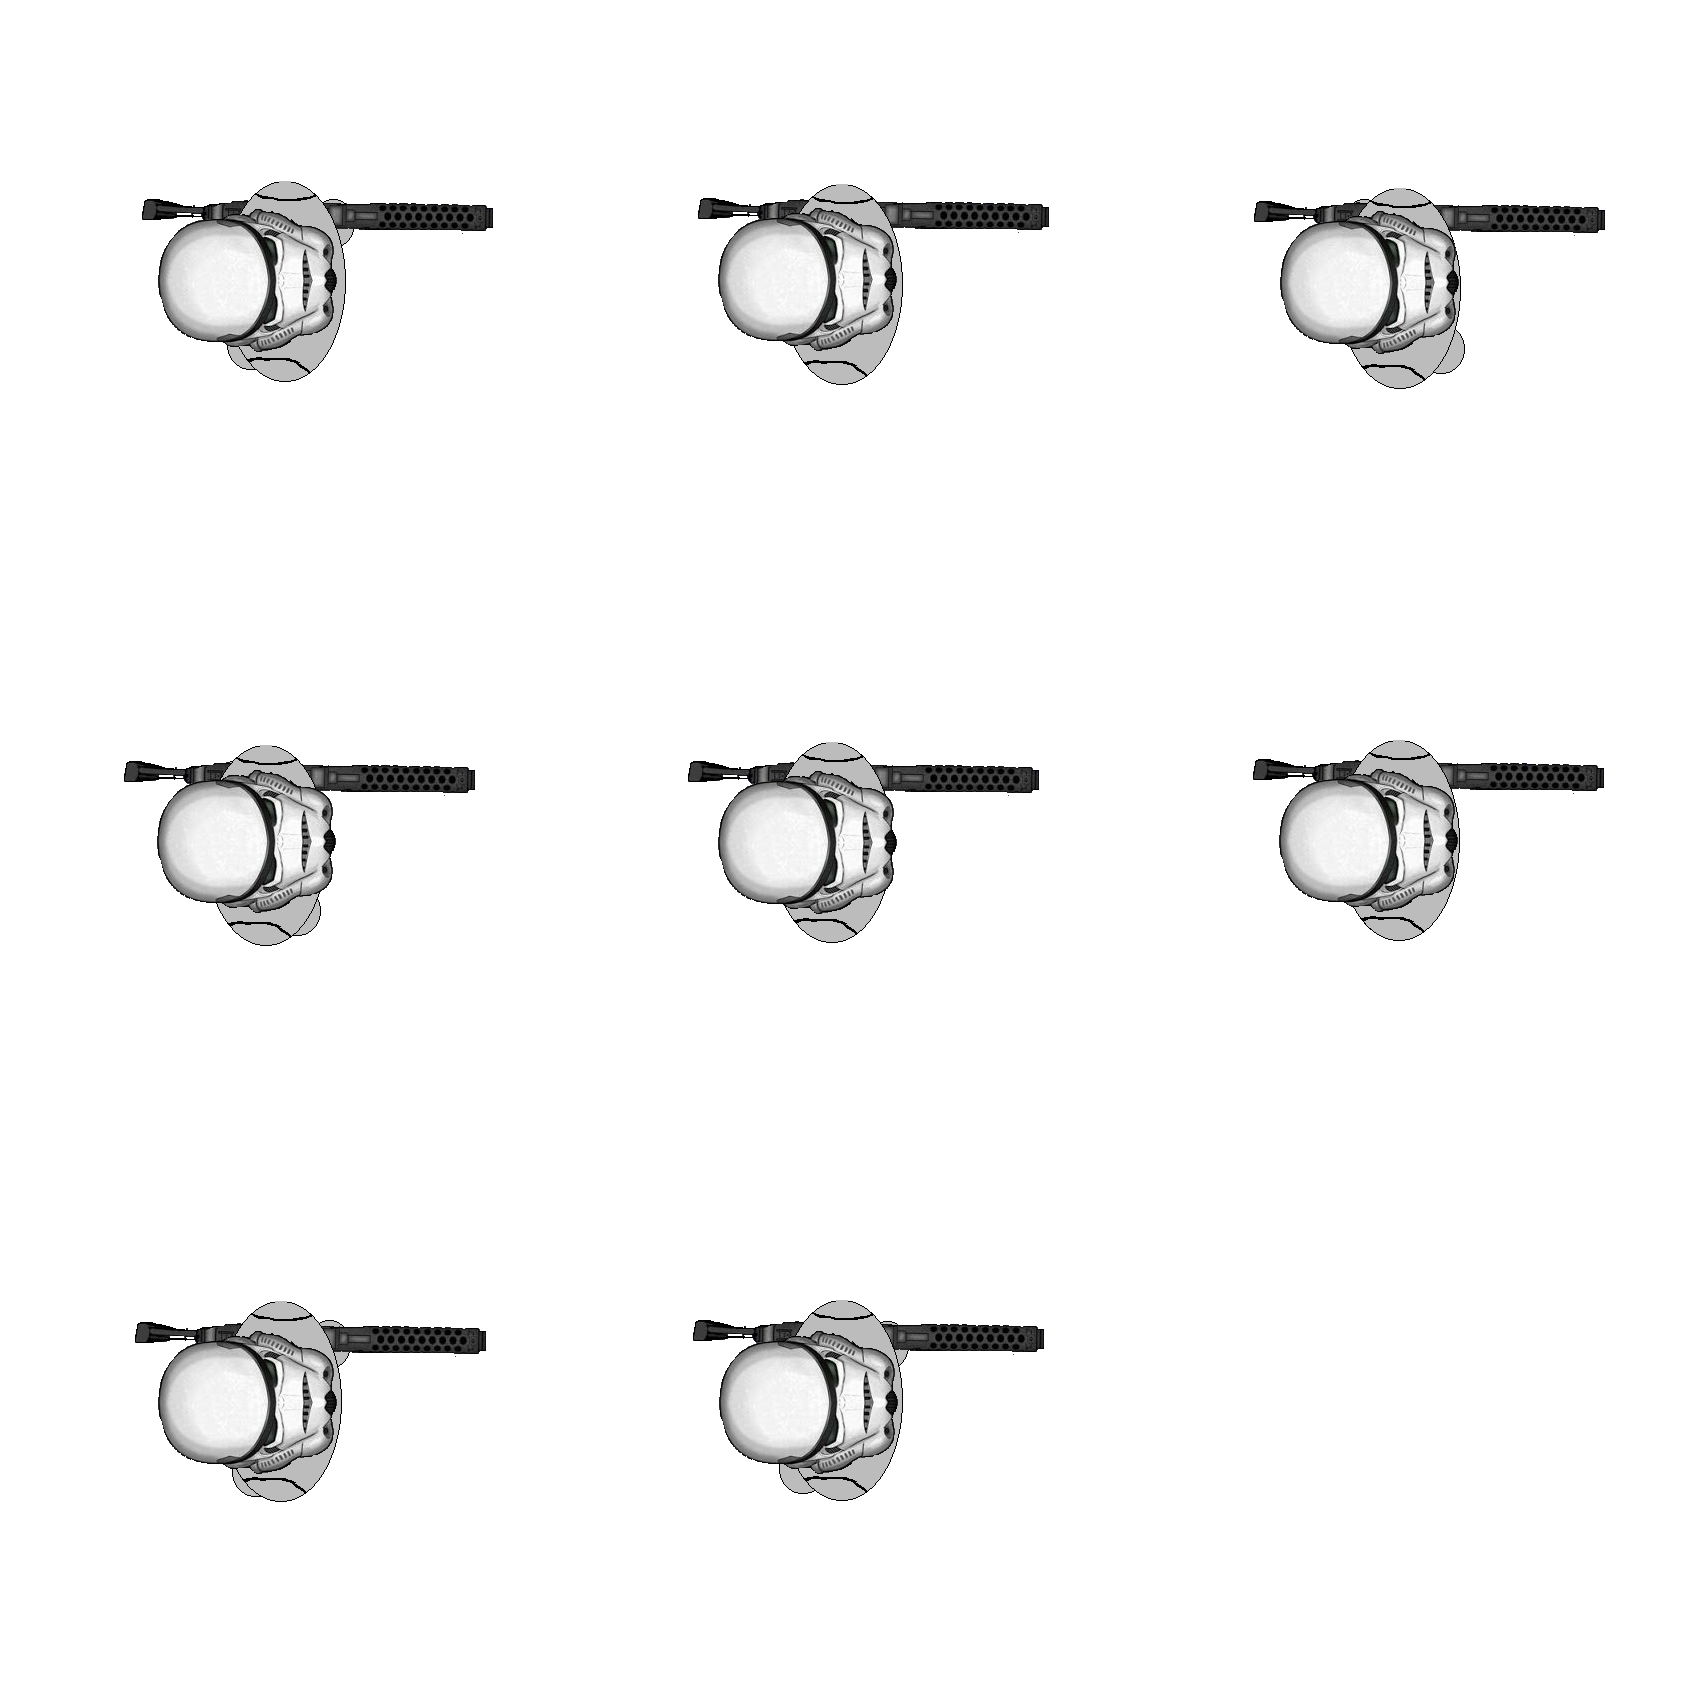
\includegraphics[width=0.5\textwidth]{pics/stormtrooper.png}
    \caption{A sprite sheet for an animation.}
    \label{fig:spritesheet}
\end{figure}

\subsubsection{Lobby}\label{sec:lobby}
We have a lobby which is the start screen you come to when starting our game, see Figure~\ref{fig:lobby}. The lobby is used to connect players together before starting a game. We have not spent much time on the lobby and it currently has only one button. The functionality of the button is that when it is pressed the player who pressed it is ready to start the game. The game will start when all the players in the lobby are ready. The lobby lacks information about how many and who has joined, so you need to coordinate with the people you want to play with and tell each other when you all have joined the game. The game does not have a limit for how many players that can play simultaneously, but with too many players the CPU usage will be too high and many packages communicated between the client and server will be dropped. Our recommendation is to play it as a maximum of 6 players.

\begin{figure}
    \centering
    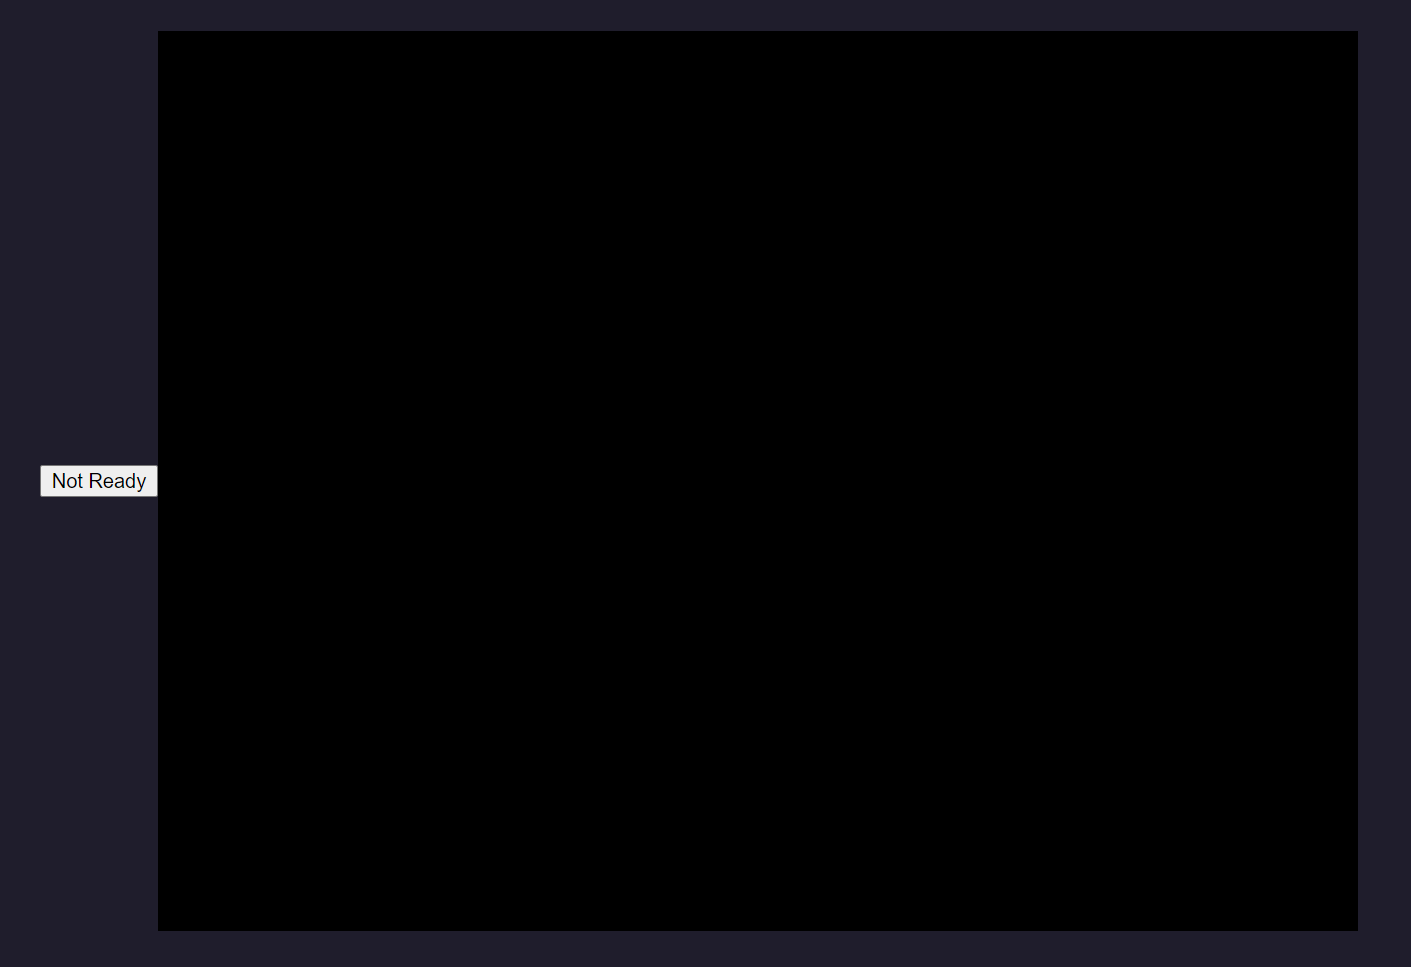
\includegraphics[width=0.5\textwidth]{pics/lobby1.png}
    \caption{The start lobby. The gray button in the left is the ready-button.}
    \label{fig:lobby}
\end{figure}

We have implemented a scoreboard where each player can see their own score and what wave they are currently playing on. When the game ends an overall scoreboard is displayed where the players can see everyone's score, see Figure~\ref{fig:scoreboard}. The game feels competitive and this is something that we are happy with.

\begin{figure}
    \centering
    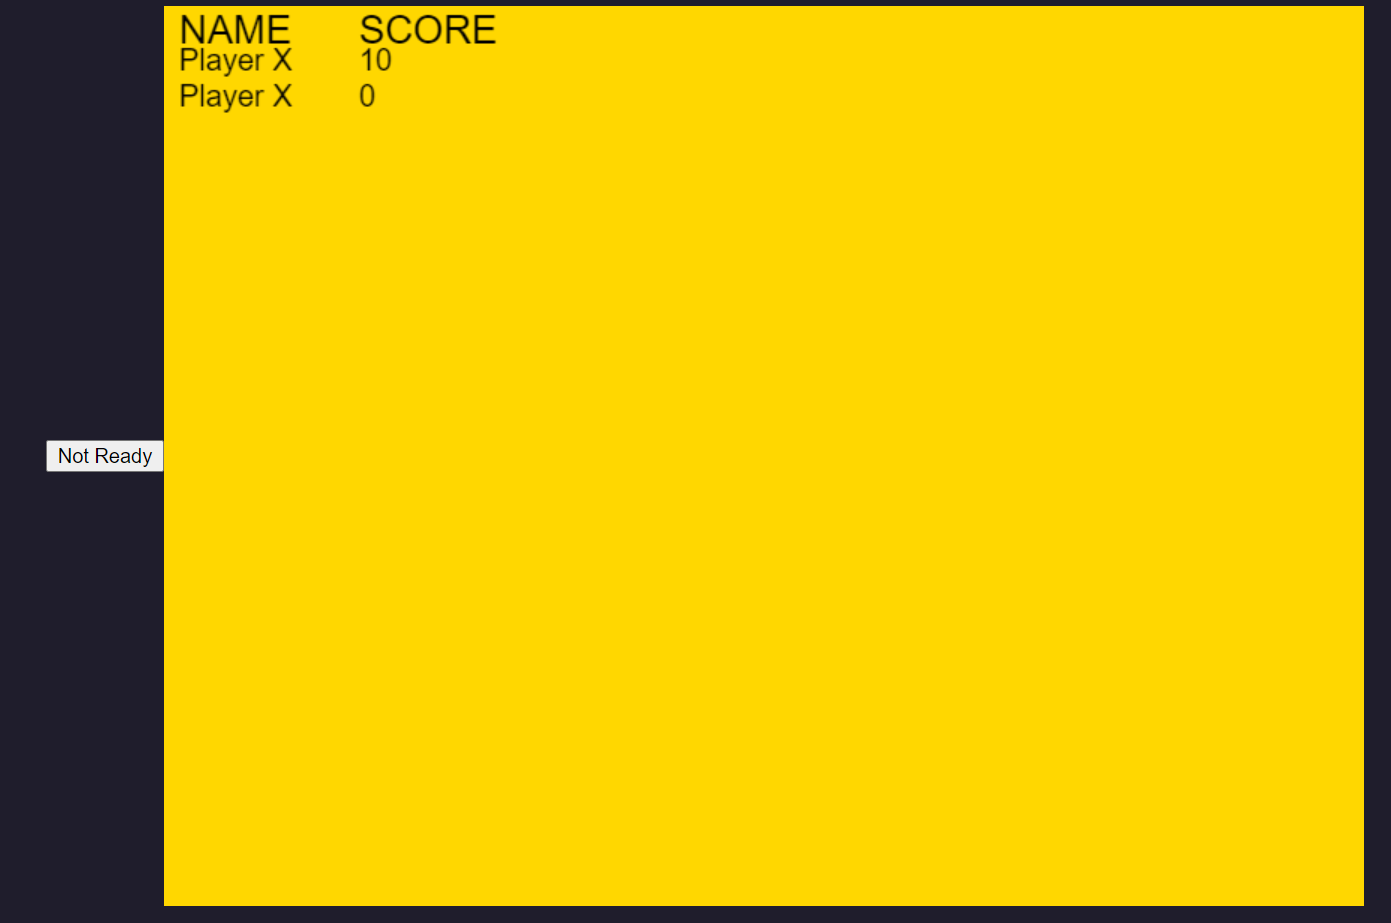
\includegraphics[width=0.5\textwidth]{pics/score1.png}
    \caption{The scoreboard when a game is finished.}
    \label{fig:scoreboard}
\end{figure}

\subsection{Testing and Quality Assurance}
When making sure that our code was up to standard we used automatic tests that was run on every code push to GitHub. These tests was both for code quality such as checking code formatting and a linter which is a code analysis tool that checks for things such as programming errors, suspicious constructs and bugs. We also had a program that tried to build the project and checked if that still was possible with the new code.

To further assure our code quality every new commit was reviewed by at least one member of the team. The reviews was not only for bug finding and making sure that the code was readable but also for giving the other members an idea of how the newly added feature worked.

The last thing we did to ensure that our code worked correctly was play testing. This means that we played the game and tried to ``break it'' in as many possible ways as we could think about.

\section{Result}

We feel like the game we created is good and we are happy with how it turned out. The game works like what we had in mind in the beginning. It is a game with mostly the core features implemented, with some small tweaks and some additional features it would feel even more complete. For example by adding different types of weapons and different enemies the game would feel much more detailed. The reason why we did not implement these features is due to shortage of time. When creating our project plan, we designed it in such a way that we would be able to end the project at many different stages and still have a complete game. This means that we focused on the core mechanics first. We are satisfied with the core structure of the game and we have built the game in a modular manner in preparation for adding more features in the future. For example it is prepared for adding multiple weapons by just adding more constants in the weapon class.

%The game feels responsive when playing. We have tested the game with different pings. With a ping of 80~ms the game is still playable. There is some delay, but not something that hinders you from playing. Even with a package drop of 50~\% the game feels great, but with some very small position jumps of the player, thanks to our client-side prediction (see Section~\ref{sec:csp}). The clients predict how the game state evolves without having to communicate with the server. Therefore dropping packages will not be as noticeable as long as the client has predicted the game state correctly.
The game is responsive even during bad network conditions. We tested with different delays and it felt good even at 80ms, which is a very high delay for a game. All players own characters moves instantly at any delay thanks to client-side prediction, but everything else is affected by the delay. At a packet drop of as high as 50\% is also pretty playable. All characters stutters some, but it works surprisingly well. Very small drop rates are not noticeable at all since the client is predicting how the game state evolves without having to communicate with the server. Therefore dropping packages will not be as noticeable as long as the client has predicted the game state correctly.

% The game became a huge success and we are counting on having more player than WoW early 2021.
% Your experience of the project from both a technical and organisation point of view -- "lessons learnt". Technical and non-technical decisions you made throughout the project. The collaboration and team work. The strategies your have followed to finish the project. Unexpected difficulties but also things that were easier than you expected. What, if anything, would you have done differently if you knew from the beginning what you know now?

The game has been shown to people with no previous experience of it. Some feedback that was given was that it is not entirely clear of how the character would be controlled, especially how to shoot. Another issue was that the test person tried to use the spawn points of the enemies as doors and repeatedly tried to walk through them. We also got some feedback that the players liked the collision mechanics between players, they felt that it encouraged cooperation. There was also some confusion about how the knock back mechanic worked and also some players did not understand that the blood on the floor was purely visual and had no impact on game play. The players also quickly figured out that they needed to use attack move if they wanted to have a chance at beating the harder levels. Attack move is when you fire a shot and move when your weapon is reloading. The players also appreciated that they got hp back and resurrected between round since that made them feel that they could take more risk and play in a less scared manner. Overall they thought it was a fun game.

\section{Future Work}
% Future work/improvements that could be done.
Temporary power-ups are common in shooter video games, e.g.\@ an increase in damage output or a reduction in damage taken from enemies. New weapons can be added to accommodate different play styles and increased variability for players. Different types of enemies can also be implemented.

Another improvement could be to compensate for network latency even more with something called lag compensation. Every client and the server have slightly different views of the game at any given point, which is a problem. Lag compensation basically means that the server rewinds its game state to make it look like it did on one of the clients. Now the server can decide whether a bullet hit an enemy in the eyes of one of the clients, making the experience better.

For enemy movement, the game computes two matrices using the Floyd-Warshall algorithm (see Section~\ref{sec:eai}). This algorithm is very time-consuming, especially for large maps, and is run on each client every time a new game starts, which introduces noticeable lag. An improvement would be to run the computation once, store the result, and send it to the clients before the game starts.

We wanted the game to work well in all web browsers, but the result performs poorly in Firefox. We are not sure why this happens, but this is something that could be looked into in the future.
%menu fix

\section{Discussion}
The collaboration between the members in the group have been good. It was easy for us to start communicating and working together since we all knew each other from before. What we learned was that having daily meetings is a great tool to make sure that everyone is aiming for the same goal. We have also used these meetings to divide work between ourselves and planning the day.

One thing that we could have done better was handling pull requests. We have worked with pull requests for every new contribution. We did not have any structure for how these should be reviewed which lead to us spending more time then necessary reviewing. Occasionally this meant that parts of the project were blocked. What we learned from this is that we should have discussed on a method for how to do this. We could have assigned some people that had their main part in reviewing pull requests to make sure that everyone always had work to do.

Another problem we had was some pull requests were huge. This was partly because we added unrelated quick-fixes and tweaks other to what we were currently working on, and partly because we were building our code base o from the ground up which means that a lot of code is added out of necessity.

One technical difficulty we encountered during the project was that our graphical library did not have support for z-indexing. Z-indexing means that it is possible to order what graphical components appear on top of each other. However, it turned out that there was a newer version of PixiJS available, PixiJS 5, that supported this feature, and we were using PixiJS 4. This was discovered quite late in the project and a lot of PixiJS 4 code had already been written. This meant that we had to modify a substantial part of the project to the newer version. What we learned from this is that it is important to check that a library has all the features you want before choosing it, something that could have saved us a lot of unnecessary work.

It was challenging to create game states that could potentially be dropped and be resumed from at any time. One example was when we wanted to record when someone made a shot. We initially stored a boolean where ``true'' meant that ``in this state this player made a shot'' and the game would draw a bullet and check whether it hit something etc. But it would be a problem if that state was dropped, then it would look like that shot never happened on the client-side. So instead we had to store at what time the shot occurred. Now if a packet is dropped the client can see that there should be a bullet visible right now (they are visible for more than one frame). So we had to think extra hard when designing the state.

Another challenge we had was with the programming language we chose to use. Most of us in the group had limited experience of TypeScript from before. This meant that we had to use much of our time early in the project to get acquainted with it. Since we wanted a web-based game it was necessary to use either JavaScript or TypeScript, and since we had more or less equal knowledge in both we chose TypeScript since it has types and we believe that it is easier to understand. The process of learning went well and we learned more and more during the whole project so it got easier the more we worked.
%technical:
%more focus on the menu
% For the final report, remember to add some text describing your experience, both technically and organisationally, including (possibly) how you went about tackling difficulties in your way.

\newpage
% \bibliographystyle{plain}
%\bibliography{bib}
\printbibliography

\end{document}
